\documentclass{standalone}
\usepackage{tikz}
\usetikzlibrary{patterns, positioning}


\begin{document}
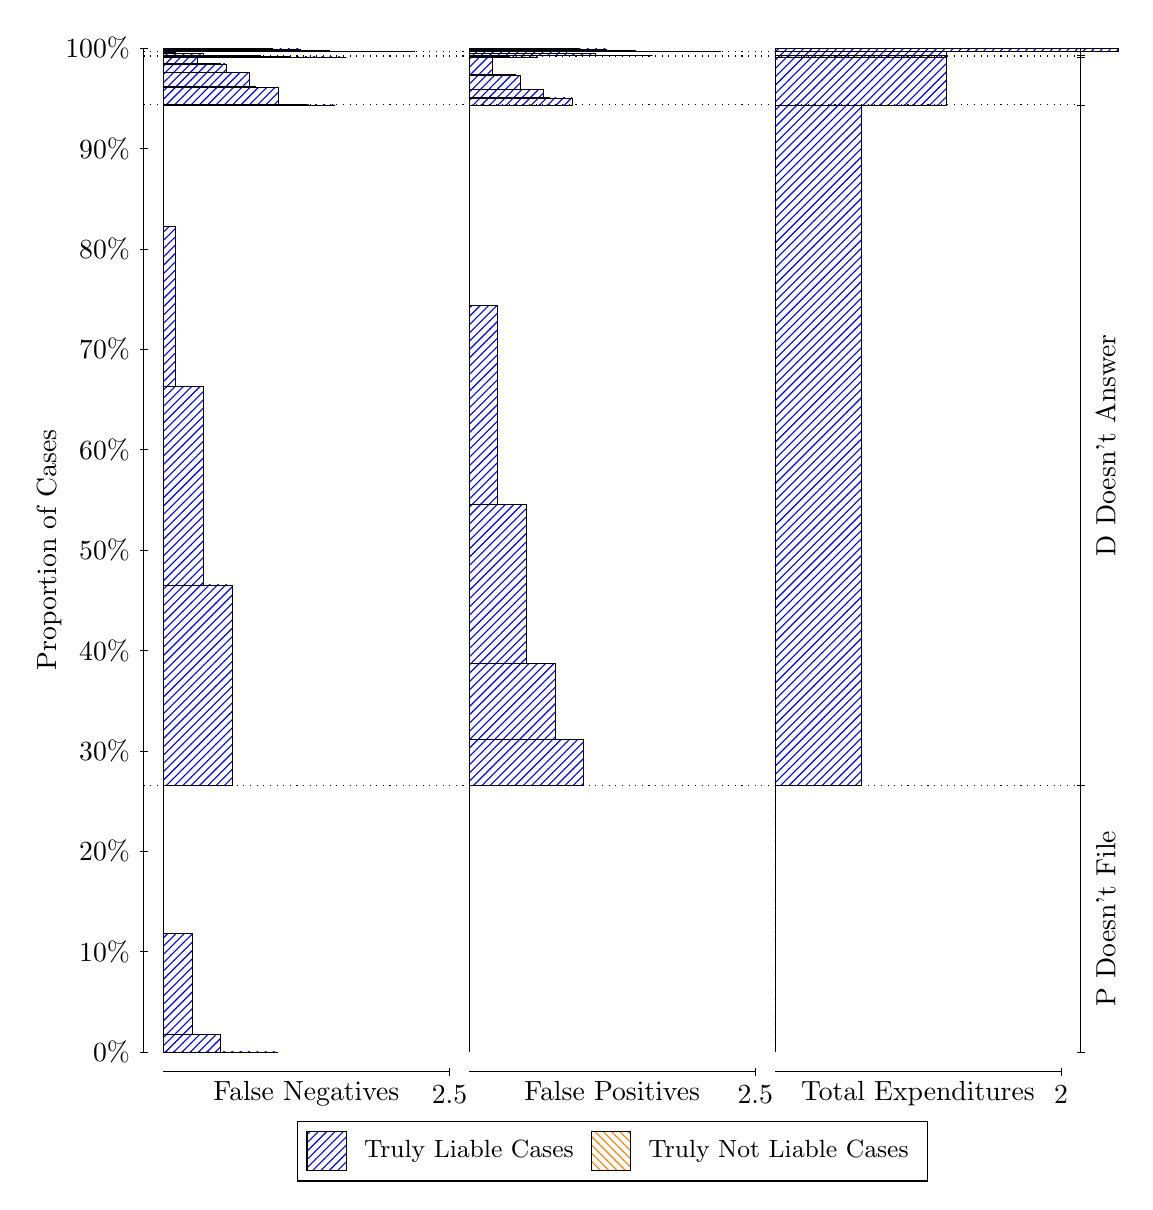
\begin{tikzpicture}
\draw[black, very thin] (1.5,1.75) -- (1.5,14.5);
\node[rotate=90, text=black, anchor=center] at (0.3, 8.125) {Proportion of Cases};
\draw[black, very thin] (1.45,1.75) -- (1.55,1.75);
\node[text=black, anchor=east] at (1.45, 1.75) {0\%};
\draw[black, very thin] (1.45,3.025) -- (1.55,3.025);
\node[text=black, anchor=east] at (1.45, 3.025) {10\%};
\draw[black, very thin] (1.45,4.3) -- (1.55,4.3);
\node[text=black, anchor=east] at (1.45, 4.3) {20\%};
\draw[black, very thin] (1.45,5.575) -- (1.55,5.575);
\node[text=black, anchor=east] at (1.45, 5.575) {30\%};
\draw[black, very thin] (1.45,6.85) -- (1.55,6.85);
\node[text=black, anchor=east] at (1.45, 6.85) {40\%};
\draw[black, very thin] (1.45,8.125) -- (1.55,8.125);
\node[text=black, anchor=east] at (1.45, 8.125) {50\%};
\draw[black, very thin] (1.45,9.4) -- (1.55,9.4);
\node[text=black, anchor=east] at (1.45, 9.4) {60\%};
\draw[black, very thin] (1.45,10.675) -- (1.55,10.675);
\node[text=black, anchor=east] at (1.45, 10.675) {70\%};
\draw[black, very thin] (1.45,11.95) -- (1.55,11.95);
\node[text=black, anchor=east] at (1.45, 11.95) {80\%};
\draw[black, very thin] (1.45,13.225) -- (1.55,13.225);
\node[text=black, anchor=east] at (1.45, 13.225) {90\%};
\draw[black, very thin] (1.45,14.5) -- (1.55,14.5);
\node[text=black, anchor=east] at (1.45, 14.5) {100\%};

\draw[black, very thin] (13.4,1.75) -- (13.4,14.5);
\draw[black, very thin] (13.35,1.75) -- (13.45,1.75);
\node[anchor=west] at (13.35, 1.75) {};
\draw[black, very thin] (13.35,5.1325) -- (13.45,5.1325);
\node[anchor=west] at (13.35, 5.1325) {};
\draw[black, very thin] (13.35,13.778) -- (13.45,13.778);
\node[anchor=west] at (13.35, 13.778) {};
\draw[black, very thin] (13.35,14.388) -- (13.45,14.388);
\node[anchor=west] at (13.35, 14.388) {};
\draw[black, very thin] (13.35,14.406) -- (13.45,14.406);
\node[anchor=west] at (13.35, 14.406) {};
\draw[black, very thin] (13.35,14.455) -- (13.45,14.455);
\node[anchor=west] at (13.35, 14.455) {};
\draw[black, very thin] (13.35,14.5) -- (13.45,14.5);
\node[anchor=west] at (13.35, 14.5) {};

\draw[black, very thin, pattern color=blue, pattern=north east lines] (1.75,1.75) rectangle (3.2033,1.75);
\draw[black, very thin, pattern color=blue, pattern=north east lines] (1.75,1.75) rectangle (2.84,1.7519);
\draw[black, very thin, pattern color=blue, pattern=north east lines] (1.75,1.7519) rectangle (2.4767,1.9775);
\draw[black, very thin, pattern color=blue, pattern=north east lines] (1.75,1.9775) rectangle (2.1133,3.2583);
\draw[black, very thin, pattern color=orange, pattern=north west lines] (1.75,3.2583) rectangle (1.75,3.2583);
\draw[black, very thin, pattern color=blue, pattern=north east lines] (1.75,3.2583) rectangle (1.75,5.1325);
\draw[black, very thin, pattern color=blue, pattern=north east lines] (1.75,5.1325) rectangle (2.622,7.6822);
\draw[black, very thin, pattern color=blue, pattern=north east lines] (1.75,7.6822) rectangle (2.2587,10.202);
\draw[black, very thin, pattern color=blue, pattern=north east lines] (1.75,10.202) rectangle (1.8953,12.231);
\draw[black, very thin, pattern color=orange, pattern=north west lines] (1.75,12.231) rectangle (1.75,12.231);
\draw[black, very thin, pattern color=blue, pattern=north east lines] (1.75,12.231) rectangle (1.75,13.778);
\draw[black, very thin, pattern color=blue, pattern=north east lines] (1.75,13.778) rectangle (3.93,13.778);
\draw[black, very thin, pattern color=blue, pattern=north east lines] (1.75,13.778) rectangle (3.6393,13.778);
\draw[black, very thin, pattern color=blue, pattern=north east lines] (1.75,13.778) rectangle (3.5667,13.783);
\draw[black, very thin, pattern color=blue, pattern=north east lines] (1.75,13.783) rectangle (3.276,13.783);
\draw[black, very thin, pattern color=blue, pattern=north east lines] (1.75,13.783) rectangle (3.2033,14.004);
\draw[black, very thin, pattern color=blue, pattern=north east lines] (1.75,14.004) rectangle (2.9127,14.01);
\draw[black, very thin, pattern color=blue, pattern=north east lines] (1.75,14.01) rectangle (2.84,14.193);
\draw[black, very thin, pattern color=blue, pattern=north east lines] (1.75,14.193) rectangle (2.5493,14.298);
\draw[black, very thin, pattern color=blue, pattern=north east lines] (1.75,14.298) rectangle (2.4767,14.3);
\draw[black, very thin, pattern color=blue, pattern=north east lines] (1.75,14.3) rectangle (2.186,14.388);
\draw[black, very thin, pattern color=orange, pattern=north west lines] (1.75,14.388) rectangle (1.75,14.388);
\draw[black, very thin, pattern color=blue, pattern=north east lines] (1.75,14.388) rectangle (4.0753,14.388);
\draw[black, very thin, pattern color=blue, pattern=north east lines] (1.75,14.388) rectangle (3.712,14.388);
\draw[black, very thin, pattern color=blue, pattern=north east lines] (1.75,14.388) rectangle (3.3487,14.397);
\draw[black, very thin, pattern color=blue, pattern=north east lines] (1.75,14.397) rectangle (2.9853,14.405);
\draw[black, very thin, pattern color=blue, pattern=north east lines] (1.75,14.405) rectangle (2.622,14.406);
\draw[black, very thin, pattern color=orange, pattern=north west lines] (1.75,14.406) rectangle (1.75,14.406);
\draw[black, very thin, pattern color=blue, pattern=north east lines] (1.75,14.406) rectangle (2.622,14.406);
\draw[black, very thin, pattern color=blue, pattern=north east lines] (1.75,14.406) rectangle (2.2587,14.428);
\draw[black, very thin, pattern color=blue, pattern=north east lines] (1.75,14.428) rectangle (1.8953,14.452);
\draw[black, very thin, pattern color=orange, pattern=north west lines] (1.75,14.452) rectangle (1.75,14.452);
\draw[black, very thin, pattern color=blue, pattern=north east lines] (1.75,14.452) rectangle (1.75,14.455);
\draw[black, very thin, pattern color=blue, pattern=north east lines] (1.75,14.455) rectangle (4.9473,14.455);
\draw[black, very thin, pattern color=blue, pattern=north east lines] (1.75,14.455) rectangle (4.584,14.455);
\draw[black, very thin, pattern color=blue, pattern=north east lines] (1.75,14.455) rectangle (4.2207,14.456);
\draw[black, very thin, pattern color=blue, pattern=north east lines] (1.75,14.456) rectangle (3.8573,14.466);
\draw[black, very thin, pattern color=blue, pattern=north east lines] (1.75,14.466) rectangle (3.494,14.489);
\draw[black, very thin, pattern color=blue, pattern=north east lines] (1.75,14.489) rectangle (3.1307,14.499);
\draw[black, very thin, pattern color=blue, pattern=north east lines] (1.75,14.499) rectangle (2.7673,14.5);
\draw[black, very thin, pattern color=blue, pattern=north east lines] (1.75,14.5) rectangle (2.404,14.5);
\draw[black, very thin, pattern color=blue, pattern=north east lines] (1.75,14.5) rectangle (2.0407,14.5);
\draw[black, very thin, pattern color=orange, pattern=north west lines] (1.75,14.5) rectangle (1.75,14.5);
\draw[black, very thin, pattern color=orange, pattern=north west lines] (5.6333,1.75) rectangle (5.6333,1.75);
\draw[black, very thin, pattern color=blue, pattern=north east lines] (5.6333,1.75) rectangle (5.6333,5.1325);
\draw[black, very thin, pattern color=orange, pattern=north west lines] (5.6333,5.1325) rectangle (7.0867,5.1325);
\draw[black, very thin, pattern color=blue, pattern=north east lines] (5.6333,5.1325) rectangle (7.0867,5.7171);
\draw[black, very thin, pattern color=blue, pattern=north east lines] (5.6333,5.7171) rectangle (6.7233,6.6802);
\draw[black, very thin, pattern color=blue, pattern=north east lines] (5.6333,6.6802) rectangle (6.36,8.709);
\draw[black, very thin, pattern color=blue, pattern=north east lines] (5.6333,8.709) rectangle (5.9967,11.229);
\draw[black, very thin, pattern color=blue, pattern=north east lines] (5.6333,11.229) rectangle (5.6333,13.778);
\draw[black, very thin, pattern color=orange, pattern=north west lines] (5.6333,13.778) rectangle (6.9413,13.778);
\draw[black, very thin, pattern color=blue, pattern=north east lines] (5.6333,13.778) rectangle (6.9413,13.867);
\draw[black, very thin, pattern color=orange, pattern=north west lines] (5.6333,13.867) rectangle (6.6507,13.867);
\draw[black, very thin, pattern color=blue, pattern=north east lines] (5.6333,13.867) rectangle (6.6507,13.869);
\draw[black, very thin, pattern color=blue, pattern=north east lines] (5.6333,13.869) rectangle (6.578,13.974);
\draw[black, very thin, pattern color=blue, pattern=north east lines] (5.6333,13.974) rectangle (6.2873,14.157);
\draw[black, very thin, pattern color=blue, pattern=north east lines] (5.6333,14.157) rectangle (6.2147,14.163);
\draw[black, very thin, pattern color=blue, pattern=north east lines] (5.6333,14.163) rectangle (5.924,14.384);
\draw[black, very thin, pattern color=blue, pattern=north east lines] (5.6333,14.384) rectangle (5.8513,14.384);
\draw[black, very thin, pattern color=blue, pattern=north east lines] (5.6333,14.384) rectangle (5.6333,14.388);
\draw[black, very thin, pattern color=orange, pattern=north west lines] (5.6333,14.388) rectangle (6.5053,14.388);
\draw[black, very thin, pattern color=blue, pattern=north east lines] (5.6333,14.388) rectangle (6.5053,14.388);
\draw[black, very thin, pattern color=blue, pattern=north east lines] (5.6333,14.388) rectangle (6.142,14.397);
\draw[black, very thin, pattern color=blue, pattern=north east lines] (5.6333,14.397) rectangle (5.7787,14.405);
\draw[black, very thin, pattern color=blue, pattern=north east lines] (5.6333,14.405) rectangle (5.6333,14.406);
\draw[black, very thin, pattern color=orange, pattern=north west lines] (5.6333,14.406) rectangle (7.9587,14.406);
\draw[black, very thin, pattern color=blue, pattern=north east lines] (5.6333,14.406) rectangle (7.9587,14.406);
\draw[black, very thin, pattern color=blue, pattern=north east lines] (5.6333,14.406) rectangle (7.5953,14.408);
\draw[black, very thin, pattern color=blue, pattern=north east lines] (5.6333,14.408) rectangle (7.232,14.432);
\draw[black, very thin, pattern color=blue, pattern=north east lines] (5.6333,14.432) rectangle (6.8687,14.455);
\draw[black, very thin, pattern color=blue, pattern=north east lines] (5.6333,14.455) rectangle (6.5053,14.455);
\draw[black, very thin, pattern color=orange, pattern=north west lines] (5.6333,14.455) rectangle (8.8307,14.455);
\draw[black, very thin, pattern color=blue, pattern=north east lines] (5.6333,14.455) rectangle (8.8307,14.455);
\draw[black, very thin, pattern color=blue, pattern=north east lines] (5.6333,14.455) rectangle (8.4673,14.455);
\draw[black, very thin, pattern color=orange, pattern=north west lines] (5.6333,14.455) rectangle (8.4673,14.455);
\draw[black, very thin, pattern color=blue, pattern=north east lines] (5.6333,14.455) rectangle (8.4673,14.455);
\draw[black, very thin, pattern color=blue, pattern=north east lines] (5.6333,14.455) rectangle (8.104,14.456);
\draw[black, very thin, pattern color=orange, pattern=north west lines] (5.6333,14.456) rectangle (8.104,14.456);
\draw[black, very thin, pattern color=blue, pattern=north east lines] (5.6333,14.456) rectangle (8.104,14.456);
\draw[black, very thin, pattern color=blue, pattern=north east lines] (5.6333,14.456) rectangle (7.7407,14.456);
\draw[black, very thin, pattern color=orange, pattern=north west lines] (5.6333,14.456) rectangle (7.7407,14.456);
\draw[black, very thin, pattern color=blue, pattern=north east lines] (5.6333,14.456) rectangle (7.7407,14.466);
\draw[black, very thin, pattern color=blue, pattern=north east lines] (5.6333,14.466) rectangle (7.3773,14.466);
\draw[black, very thin, pattern color=orange, pattern=north west lines] (5.6333,14.466) rectangle (7.3773,14.466);
\draw[black, very thin, pattern color=blue, pattern=north east lines] (5.6333,14.466) rectangle (7.3773,14.489);
\draw[black, very thin, pattern color=blue, pattern=north east lines] (5.6333,14.489) rectangle (7.014,14.499);
\draw[black, very thin, pattern color=blue, pattern=north east lines] (5.6333,14.499) rectangle (6.6507,14.5);
\draw[black, very thin, pattern color=blue, pattern=north east lines] (5.6333,14.5) rectangle (6.2873,14.5);
\draw[black, very thin, pattern color=blue, pattern=north east lines] (5.6333,14.5) rectangle (5.924,14.5);
\draw[black, very thin, pattern color=orange, pattern=north west lines] (9.5167,1.75) rectangle (9.5167,1.75);
\draw[black, very thin, pattern color=blue, pattern=north east lines] (9.5167,1.75) rectangle (9.5167,5.1325);
\draw[black, very thin, pattern color=orange, pattern=north west lines] (9.5167,5.1325) rectangle (10.607,5.1325);
\draw[black, very thin, pattern color=blue, pattern=north east lines] (9.5167,5.1325) rectangle (10.607,13.778);
\draw[black, very thin, pattern color=orange, pattern=north west lines] (9.5167,13.778) rectangle (11.697,13.778);
\draw[black, very thin, pattern color=blue, pattern=north east lines] (9.5167,13.778) rectangle (11.697,14.388);
\draw[black, very thin, pattern color=orange, pattern=north west lines] (9.5167,14.388) rectangle (11.697,14.388);
\draw[black, very thin, pattern color=blue, pattern=north east lines] (9.5167,14.388) rectangle (11.697,14.406);
\draw[black, very thin, pattern color=orange, pattern=north west lines] (9.5167,14.406) rectangle (11.697,14.406);
\draw[black, very thin, pattern color=blue, pattern=north east lines] (9.5167,14.406) rectangle (11.697,14.455);
\draw[black, very thin, pattern color=orange, pattern=north west lines] (9.5167,14.455) rectangle (13.877,14.455);
\draw[black, very thin, pattern color=blue, pattern=north east lines] (9.5167,14.455) rectangle (13.877,14.456);
\draw[black, very thin, pattern color=orange, pattern=north west lines] (9.5167,14.456) rectangle (13.877,14.456);
\draw[black, very thin, pattern color=blue, pattern=north east lines] (9.5167,14.456) rectangle (13.877,14.5);
\draw[black, dotted] (1.5,5.1325) -- (13.4,5.1325);
\draw[black, dotted] (1.5,13.778) -- (13.4,13.778);
\draw[black, dotted] (1.5,14.388) -- (13.4,14.388);
\draw[black, dotted] (1.5,14.406) -- (13.4,14.406);
\draw[black, dotted] (1.5,14.455) -- (13.4,14.455);
\draw[black, very thin] (1.75,1.5) -- (5.3833,1.5);
\node[text=black, anchor=north] at (3.5667, 1.5) {False Negatives};
\draw[black, very thin] (5.3833,1.45) -- (5.3833,1.55);
\node[text=black, anchor=north] at (5.3833, 1.45) {2.5};

\draw[black, very thin] (5.6333,1.5) -- (9.2667,1.5);
\node[text=black, anchor=north] at (7.45, 1.5) {False Positives};
\draw[black, very thin] (9.2667,1.45) -- (9.2667,1.55);
\node[text=black, anchor=north] at (9.2667, 1.45) {2.5};

\draw[black, very thin] (9.5167,1.5) -- (13.15,1.5);
\node[text=black, anchor=north] at (11.333, 1.5) {Total Expenditures};
\draw[black, very thin] (13.15,1.45) -- (13.15,1.55);
\node[text=black, anchor=north] at (13.15, 1.45) {2};

\node[text=black, centered, rotate=90] at (13.72, 3.4413) {P Doesn't File};
\node[text=black, centered, rotate=90] at (13.72, 9.4555) {D Doesn't Answer};





\draw (7.449999999999999,1.5) node[draw=none] (baseCoordinate) {};
\begin{scope}[align=center]
        \matrix[scale=0.5, draw=black, below=0.5cm of baseCoordinate, nodes={draw}, column sep=0.1cm]{
            \node[rectangle, draw, minimum width=0.5cm, minimum height=0.5cm, pattern color=blue, pattern=north east lines] {}; &
            \node[draw=none, font=\small, text=black] (B) {Truly Liable Cases}; &
            \node[rectangle, draw, minimum width=0.5cm, minimum height=0.5cm, pattern color=orange, pattern=north west lines] {}; &
            \node[draw=none, font=\small, text=black] (B) {Truly Not Liable Cases}; \\
            };
\end{scope}

\end{tikzpicture}
\end{document}